\scanpage{51}
\handwritten{$\unsure{\rho|p}$}

\handwritten{\figure{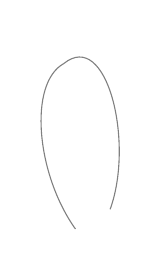
\begin{tikzpicture}[x=1cm,y=1cm]
\draw[thin,gray] (0,0) .. controls (-.5,.7) and (-.6,1.85) .. (-.15,2.1) .. controls (.4,2.55) and (.75,1.1) .. (.44,.25);
\end{tikzpicture}}}

\handwritten{\figure{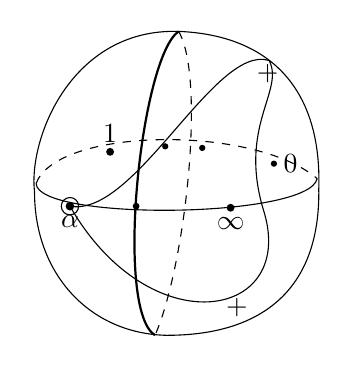
\begin{tikzpicture}[x=1cm,y=1cm]
\draw (0,1.9) .. controls (-1.36,1.94) and (-1.91,.54) .. (-1.83,-.14) .. controls (-1.83,-1.18) and (-1.13,-1.94) .. (-.15,-1.96) .. controls (1.1,-1.96) and (1.8,-1.34) .. (1.78,-.1) .. controls (1.82,1.14) and (1.19,1.85) .. (0,1.9);
\draw[dashed] (-1.81,-.03) .. controls (-1.54,.68) and (.95,.72) .. (1.76,.03);
\draw (1.76,.03) .. controls (1.65,-.48) and (-1.8,-.51) .. (-1.81,-.03);
\draw[thick] (0,1.9) .. controls (-.48,1.57) and (-.82,-1.63) .. (-.3,-1.96);
\draw[dashed] (0,1.9) .. controls (.35,1.3) and (.08,-1.1) .. (-.3,-1.96);
\draw[thin] (-1.38,-.32) .. controls (-.55,-.47) and (.46,1.75) .. (1.15,1.53) .. controls (1.35,1.14) and (.74,.69) .. (1.09,-.41) .. controls (1.48,-1.77) and (-.37,-2.08) .. (-1.38,-.32);
\draw (-1.38,-.32) circle (.11);
\fill (-1.38,-.32) circle (.055) node[below] {$\alpha$};
\fill (-.87,.37) circle (.05) node[above] {$1$};
\fill (1.21,.22) circle (.04) node[right] {$0$};
\fill (.66,-.34) circle (.05) node[below] {$\infty$};
\fill (-.54,-.32) circle (.043); \fill (-.17,.44) circle (.04); \fill (.3,.42) circle (.04);
\node at (1.13,1.36) {$+$}; \node at (.74,-1.61) {$+$};
\end{tikzpicture}}}

\handwritten{$\mathscr T_{0,4}^{+!}\simeq\Pi_{0,3}\deleted{\unsure{\simeq}}$}

\handwritten{\diagram{\begin{tikzcd}[ampersand replacement=\&,column sep=small,row sep=small]
1\arrow[r]\&\Pi_{0,3}\arrow[r]\arrow[d,equal]\&\mathscr T^+_{0,4}\arrow[r]\arrow[d,"\mathrm{cart}"]\&\unsure{\mathfrak S|\mathscr G}_4\arrow[r]\arrow[d,"\mathrm{can}"]\&1\\
1\arrow[r]\&\Pi_{0,3}\arrow[r]\&\mathscr T^+_{0,1}/\pm1\arrow[r]\arrow[d,phantom,sloped,"\simeq"]\&\mathfrak S_3\arrow[r]\arrow[d,phantom,sloped,"\simeq"]\&1\\
\&\&\mathrm{Sl}(2,\mathbb Z)/\pm1\&\mathrm{Sl}(2,\mathbb Z/2\mathbb Z)\&
\end{tikzcd}}}

\handwritten{\diagram{\begin{tikzcd}[ampersand replacement=\&,row sep=small]
\mathscr T^{+\unsure{/|\prime}}_{0,4}\simeq\mathscr T^+_{0,1}/\pm1\arrow[d,phantom,sloped,"\simeq"]\\
\mathrm{Sl}(2,\mathbb Z)/\pm1
\end{tikzcd}}}

\handwritten{\diagram{\begin{tikzcd}[ampersand replacement=\&,column sep=small,row sep=tiny]
0\arrow[r]\&\Pi_{0,3}\arrow[r]\&\mathscr T^+_{0,1}\arrow[r]\arrow[d,equal]\&\deleted{\unsure{\mathbb Z/2\mathbb Z|\mathfrak S}}\widetilde{\mathfrak S}_3\arrow[r,dash]\arrow[d,equal]\&1\\
\deleted{\unsure{e_1,e_2,e_1+e_2|e_1,e_2,e_1,e_2}}\&\&\mathrm{Sl}(2,\mathbb Z)\&\mathrm{Sl}(2,\mathbb Z/4\mathbb Z)/\unsure{---}\&
\end{tikzcd}}}

\handwritten{\diagram{\begin{tikzcd}[ampersand replacement=\&,row sep=small,column sep=small]
\mathrm{Sl}(2,\mathbb Z)/\underbrace{(\pm1.\mathbb Z)}_{\text{\uline{Borel}}}\simeq\&
\unsure{\mathbb P^1(\mathbb Z)|\mathbb P^1_{\mathbb Z}}\arrow[d]\&
{}\simeq\mathbb P^1(\mathbb Q)\\
\&\mathbb P^1(\mathbb Z/2\mathbb Z)\&
\end{tikzcd}}}

\handwritten{$\mathscr T\qquad\Pi_{0,3}$}

\handwritten{\figure{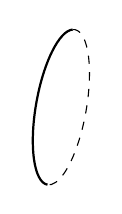
\begin{tikzpicture}
\draw[thick,rotate=-10] (0,0) arc[start angle=-90,end angle=-265,x radius=.32cm,y radius=1cm];
\draw[dashed,rotate=-10] (-.028,1.996) arc[start angle=95,end angle=-90,x radius=.32cm,y radius=1cm];
\end{tikzpicture}}}

\handwritten{$\unsure{\mathfrak{gl}|\mathrm{gl}|\mathrm{Gl}}(2,F_2)$}

\handwritten{\[
\begin{aligned}
&&l_0\,l_1\,l_2\,l_3&=1\\
l_0\,l_1\,l_\infty&=1\\
l'_{\unsure{\infty|0}}\,l'_2\,l'_3&=1&&l_\infty=l'_\infty
\end{aligned}
\]}

\handwritten{\[
\begin{aligned}
&\mathscr T S D\\
&\mathscr T S\qquad\mathscr T D&&\mathbb T S D\\
&\mathscr T&&\mathbb T S\quad\mathbb T D\\
&&&\mathbb T
\end{aligned}
\]}

\handwritten{$\mathscr T_{0,4}^{+\prime}$}

\handwritten{\begin{tabular}{ll}
groupoïdes & $\mathscr T$\\
groupes & $T$\\
multiplicités & $M$\\
\uline{espace} de T & $\widetilde M$
\end{tabular}}

\handwritten{\[
\begin{aligned}
&\mathscr T^+\ \deleted{\unsure{\mathscr T}}\\
&T^+,T^!,T^{+!},\ T^/,T^{/+}
\end{aligned}
\]}

\handwritten{$\mathrm{Gl}(2,\mathbb Z)/\mathbb Z^*$}

\handwritten{\diagram{\begin{tikzcd}[ampersand replacement=\&,column sep=small,row sep=small]
1\arrow[r]\&\unsure{\pi|\Pi}_{g,\nu-1}\arrow[r]\&\mathbb T_{g,\nu}\arrow[r]\arrow[d,phantom,sloped,"\simeq"]\&\underbrace{\mathbb T_{g,\nu-1}}_{X_{g,\nu-1}}\arrow[r]\&1\\
\&\&\pi_1(\mathscr X_{g,\nu-1},\mathbb T_{g,\nu-1};s_\nu)\&\&
\end{tikzcd}}
\[
X_{g,\nu-1}\subset\mathscr X
\]}

\handwritten{\figure{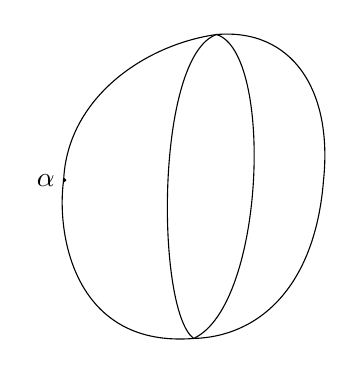
\begin{tikzpicture}
\draw[thin] (0,0) .. controls (-1.5,-.12) and (-1.75,1.3) .. (-1.65,2.02) .. controls (-1.6,3.05) and (-.63,3.73) .. (.29,3.86) .. controls (1.24,3.94) and (1.77,3.17) .. (1.65,2.01) .. controls (1.54,.62) and (.8,.02) .. (0,0);
\draw (0,0) .. controls (-.48,.36) and (-.49,3.58) .. (.29,3.86) .. controls (1.02,3.64) and (.91,.42) .. (0,0);
\fill (-1.64,2.01) circle (.025) node[left] {$\alpha$};
\end{tikzpicture}}}

\handwritten{$\deleted{\unsure{\mathscr M}}M_{g,\nu}\;-$}

\handwritten{$\Pi_{0,3}\qquad\mathfrak S_3$}

\handwritten{\figure{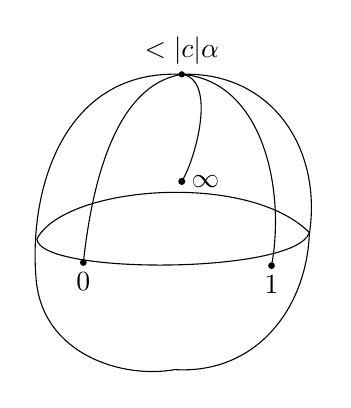
\begin{tikzpicture}
\draw (.12,1.83) .. controls (-1.36,1.9) and (-1.83,.4) .. (-1.73,-.77) .. controls (-1.65,-1.73) and (-.63,-2.04) .. (.03,-1.92) .. controls (1.07,-1.98) and (1.7,-1.14) .. (1.74,-.2) .. controls (1.91,.9) and (1.25,1.87) .. (.12,1.83);
\draw[thin] (-1.72,-.26) .. controls (-1.36,.42) and (.97,.6) .. (1.74,-.18) .. controls (1.57,-.71) and (-1.69,-.72) .. (-1.72,-.26);
\draw (-1.13,-.56) .. controls (-.97,.9) and (-.55,1.72) .. (.12,1.83) .. controls (1.15,1.75) and (1.44,.37) .. (1.26,-.6);
\draw (.12,1.83) .. controls (.57,1.77) and (.3,.76) .. (.12,.47);
\fill (.12,1.83) circle (.04) node[above] {$\unsure{<|c|\alpha}$};
\fill (.12,.47) circle (.045) node[right] {$\infty$};
\fill (-1.13,-.56) circle (.043) node[below] {$0$}; \fill (1.26,-.6) circle (.043) node[below] {$1$};
\end{tikzpicture}}}

% printed form
{\tiny
\begin{verbatim}
//*   CRAY2   0369       I
           00000000      00000000      00000000      00000000
         0000000000    0000000000    0000000000    0000000000
       00      0000  00      0000  00      0000  00      0000
      00     00 00  00     00 00  00     00 00  00     00 00
     00    00  00  00    00  00  00    00  00  00    00  00
    00   00   00  00   00   00  00   00   00  00   00   00
   00  00    00  00  00    00  00  00    00  00  00    00
  00 00     00  00 00     00  00 00     00  00 00     00
 0000      00  0000      00  0000      00  0000      00
000       00  000       00  000       00  000       00
0000000000    0000000000    0000000000    0000000000
00000000      00000000      00000000      00000000

 CCCCCCCCCC   RRRRRRRRRRR    AAAAAAAAAA   YY        YY   2222222222
CCCCCCCCCCCC  RRRRRRRRRRRR  AAAAAAAAAAAA  YY        YY  222222222222
CC        CC  RR        RR  AA        AA   YY      YY   22        22
CC            RR        RR  AA        AA    YY    YY              22
CC            RR        RR  AA        AA     YY  YY               22
CC            RRRRRRRRRRRR  AAAAAAAAAAAA      YYYY               22
CC            RRRRRRRRRRR   AAAAAAAAAAAA       YY              22
CC            RR    RR      AA        AA       YY            22
CC            RR     RR     AA        AA       YY          22
CC        CC  RR      RR    AA        AA       YY        22
CCCCCCCCCCCC  RR       RR   AA        AA       YY       222222222222
 CCCCCCCCCC   RR        RR  AA        AA       YY       222222222222

****A  START  JOB  369  CRAY2                         ROOM        3.45.56 PM 16 AUG 82  R6.PR1    SYS JES2  JOB  369  START  A****
****A  START  JOB  369  CRAY2                         ROOM        3.45.56 PM 16 AUG 82  R6.PR1    SYS JES2  JOB  369  START  A****
****A  START  JOB  369  CRAY2                         ROOM        3.45.56 PM 16 AUG 82  R6.PR1    SYS JES2  JOB  369  START  A****
****A  START  JOB  369  CRAY2                         ROOM        3.45.56 PM 16 AUG 82  R6.PR1    SYS JES2  JOB  369  START  A****
****A  START  JOB  369  CRAY2                         ROOM        3.45.56 PM 16 AUG 82  R6.PR1    SYS JES2  JOB  369  START  A****
****A  START  JOB  369  CRAY2                         ROOM        3.45.56 PM 16 AUG 82  R6.PR1    SYS JES2  JOB  369  START  A****

DERNIERE MISE A JOUR DE JOURNAL : 11-08-82
ATTENTION .............
   ]      1. UNE MODIFICATION SYSTEME NOUS CONTRAINDRA A DETRUIRE
   ]         LE CONTENU DU DISQUE-SPOOL LE MARDI 17 AOUT A 6 HEURES
   ]         VEUILLEZ RECUPERER VOS SORTIES EN ATTENTE AVANT CETTE
   ]         DATE. MERCI DE VOTRE COMPREHENSION.
   ]      2. UN ARRET EXCEPTIONNEL POUR PREPARER L'ARRIVEE DE NOUVELLES
   ]         UNITES AURA LIEU DU VENDREDI 20 AOUT A 17H 30 AU LUNDI
   ]         23 AOUT A 8H.
\end{verbatim}
}

% archive sheet number: 53
